%--------------------------------------------------------------------------------------------------
% 
\chapter{Big Data Framework based on Lambda Architecture}
\label{ch:big_data_framework}
%--------------------------------------------------------------------------------------------------

\epigraph{Architecture is not about space, nor about containment. It's about relationships, about connections, about extending our experience into new territories.}{\textit{Juhani Pallasmaa}}

This chapter describes an implementation as well as evaluation of the lambda architecture (see Figure \ref{fig:the_big_picture}) in the water management scenario.
The first section focuses on the implementation of the architecture, whereas the second section focuses on the evaluation.

\section{Framework}

% introducing the paper
\begin{quote}
In this section, we introduce the paper entitled \textit{Computer Architectures for Incremental Learning in Water Management}, authored by Klemen Kenda, Nikos Mellios, Matej Senožetnik, and Petra Pergar. 
This paper has been published in the Sustainability~\cite{kenda:2022:water-framework}.
Klemen Kenda contributed significantly to conceptualization and methodology development presented in this paper. 
He contributed to software development, design and implementation of evaluation.
He lead the writing of the paper and also contributed to visualizations.
\end{quote}

The paper presents an implementation of the platform based on the lambda architecture and modules described in this publication.
The platform is coined Water Management Analytical Platform (WMAP) and serves the data and modeling needs in the water sector.
Implementation is steered towards solving real-world issues such as ingestion and wrangling of heterogeneous live data streams, forming model results on the live data and building custom solutions on top of standard predictive/anomaly detection services.
The suggested framework builds upon established big data (lambda) architectures and offers an effective approach to address data-driven modeling within the water management sector. 
The primary enhancement lies in the speed pillar (online analytics) of the architecture. 
Here, we introduce heterogeneous data fusion across a range of data streams to deliver real-time data-driven modeling and prediction services more efficiently.

The architecture described above has been widely used in the H2020 NAIADES project.
The Figure \ref{fig:naiades_architecture} illustrates the implementation of this architecture.
The NAIADES project consisted of three pilot sites, each addressing slightly different issues related to flower beds watering, saline water intrusion in water distribution networks, water consumption, and water leakage. 
In this implementation, data enters the system through FI-WARE adapters in the Data Layer on the left side of the figure. 
Data, as well as various analytics results such as feature vectors and predictions, are then exchanged between components using a pub/sub mechanism (via Kafka topics). 
The architecture includes two layers to cater to different analytics needs, namely basic and advanced analytics. 
The basic analytics layer comprises general-purpose components like data fusion and enrichment (described in Chapter \ref{ch:data-fusion}), forecasting, and anomaly detection.
On the other hand, the advanced analytics layer requires more domain-specific knowledge, and its components are tailored to specific use cases.
An instance of this is the detection of leaks at the advanced analytics level, which is activated by services for anomaly detection provided by the basic analytics. 
The identification of the specific location of leaks is carried out through a leakage group finder that combines the results of physical models produced with EPANET with the capabilities of machine learning. 
Ultimately, the use of genetic algorithms facilitates the strategic placement of sonic sensors for precise leak detection.
In addition to these analytics components, the WMAP implementation also includes other software components necessary for maintaining and troubleshooting the machine learning pipelines. 
Finally, all analytics results are sent back to the data layer and inserted into the NAIADES platform via FI-WARE adapters, where they are made available to the user.

\begin{figure}
    \centering
    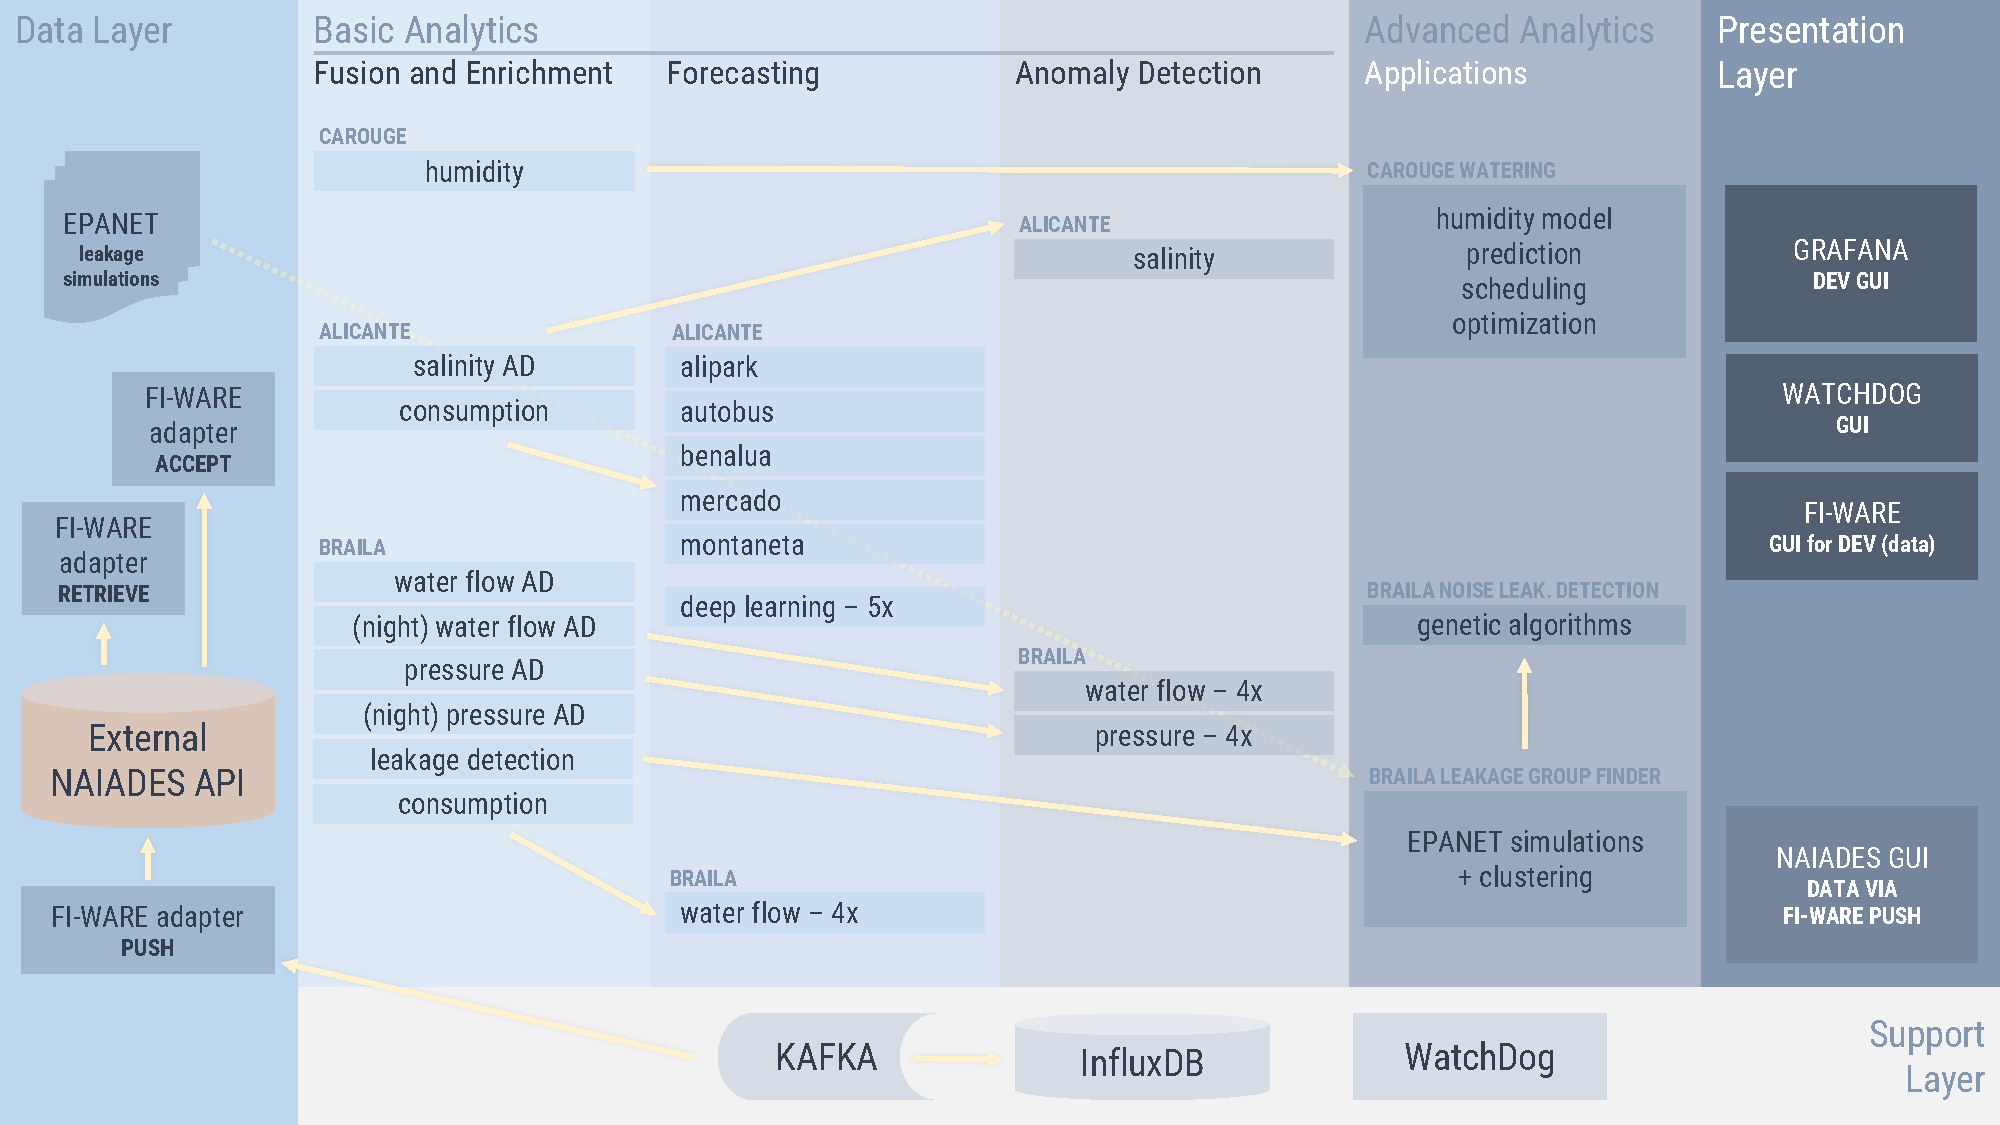
\includegraphics[width=15cm]{figures/architecture-naiades.pdf}
    \caption{Implementation of the WMAP architecture in the H2020 NAIADES project.}
    \label{fig:naiades_architecture}
\end{figure}

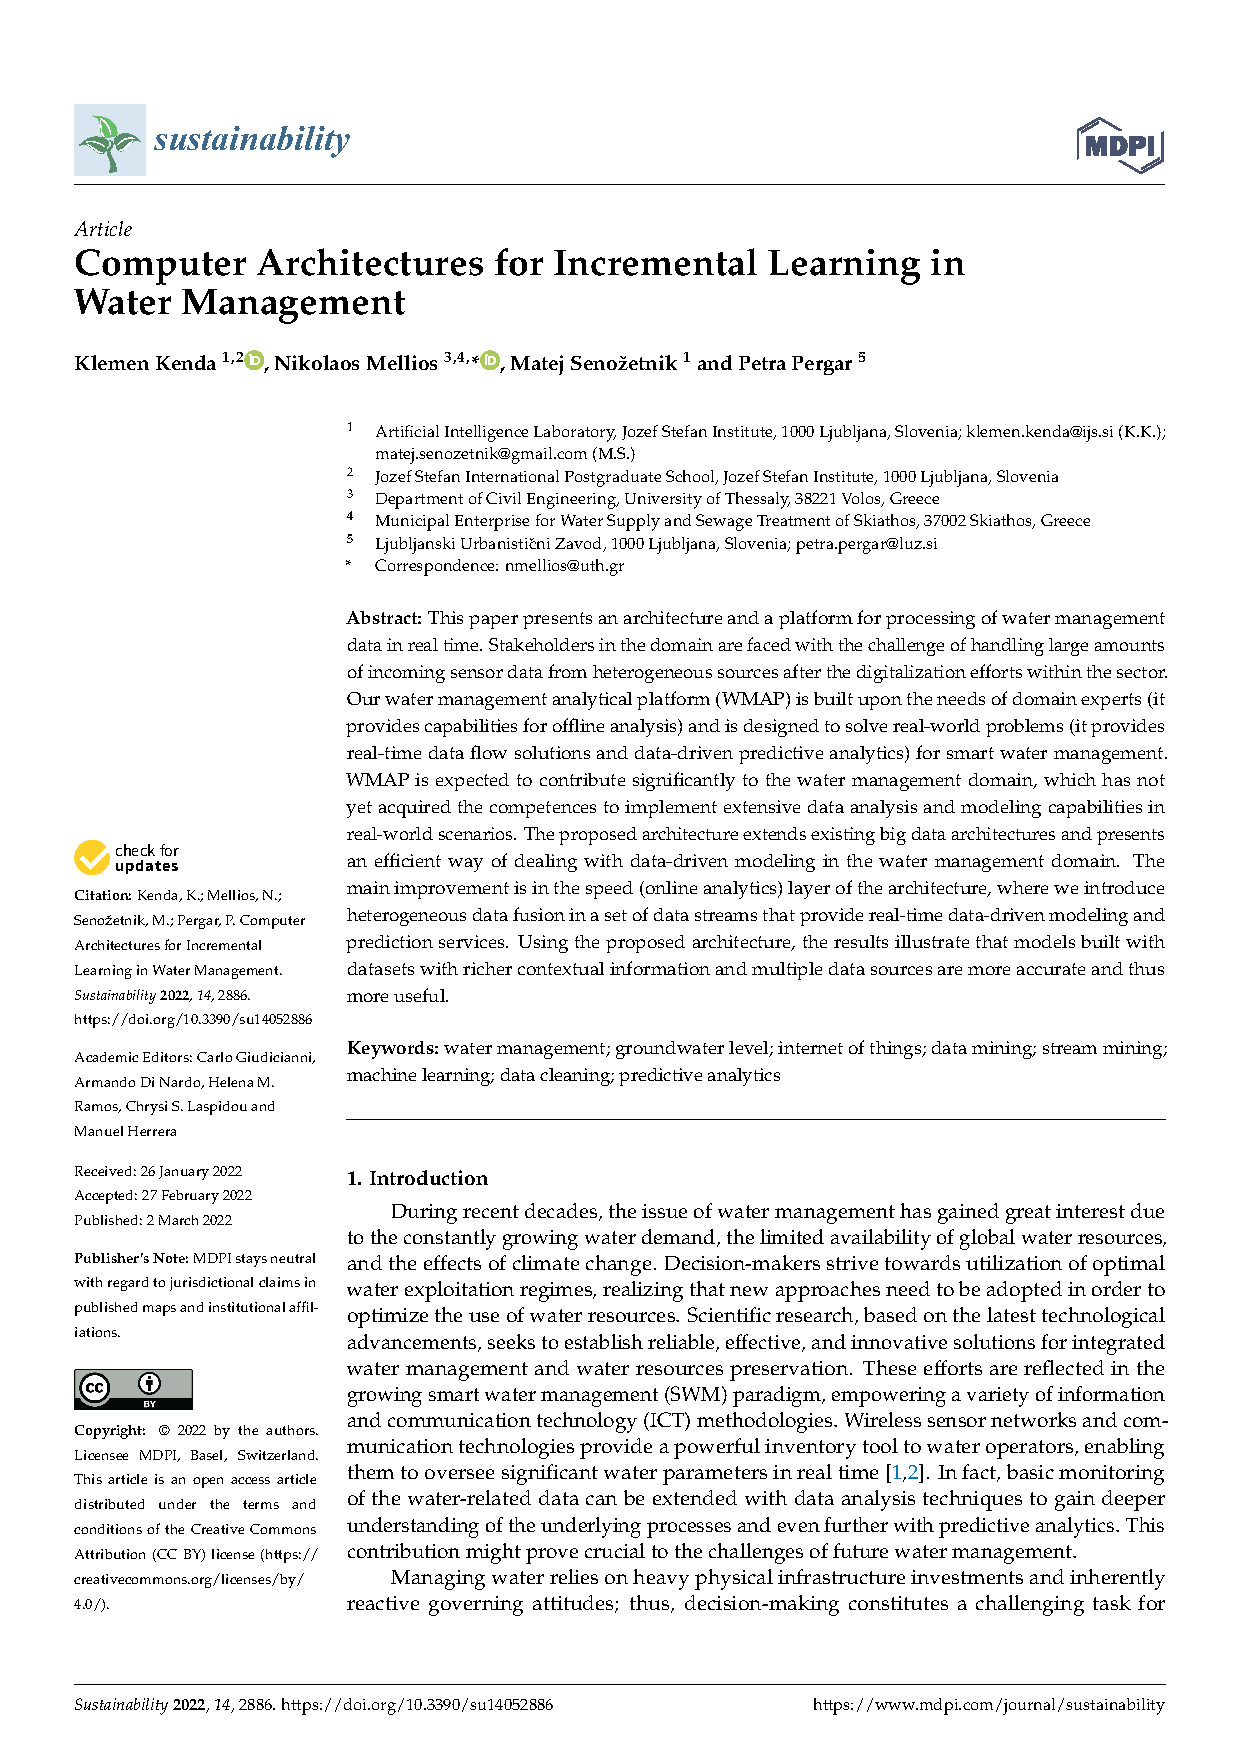
\includepdf[pages=-]{papers/architectures.pdf}


\section{Incremental Learning}
\label{section:incremental_learning}

% introducing the paper
\begin{quote}
This chapter presents the paper titled \textit{Usage of statistical modeling techniques in surface and groundwater level prediction} by Klemen Kenda, Jože Peternelj, Nikos Mellios, Dimitris Kofinas, Matej Čerin, and Jože Rožanec.
This paper has been published in the Journal of Water Supply: Research and Technology-AQUA~\cite{kenda:2020:water-modeling}.
Klemen Kenda contributed significantly to conceptualization and methodology development presented in this paper. 
He contributed to software development, design and implementation of evaluation.
He lead the writing of the paper and also contributed to visualizations.
\end{quote}

The lambda architecture, combined with the streaming sensor fusion module, can create feature vectors needed for machine learning methodologies that include a number of contextual and derived features from all the available streaming data sources.
Moreover, the system can generate the feature vectors needed for inference and also for learning (equipped with labels) on the fly.
In such a system - inherently - incremental learning approaches can be utilized with ease.

The presented paper evaluates more than 20 algorithms (among them 5 incremental algorithms) on two predictive tasks in water sector.
We built solutions for predicting water levels of surface and groundwater levels.
The main finding of the paper is that (at least for the two problems analysed) batch models are superior to the incremental ones.
Incremental models are still good enough in certain scenarios and could be used in certain large-scale operations.

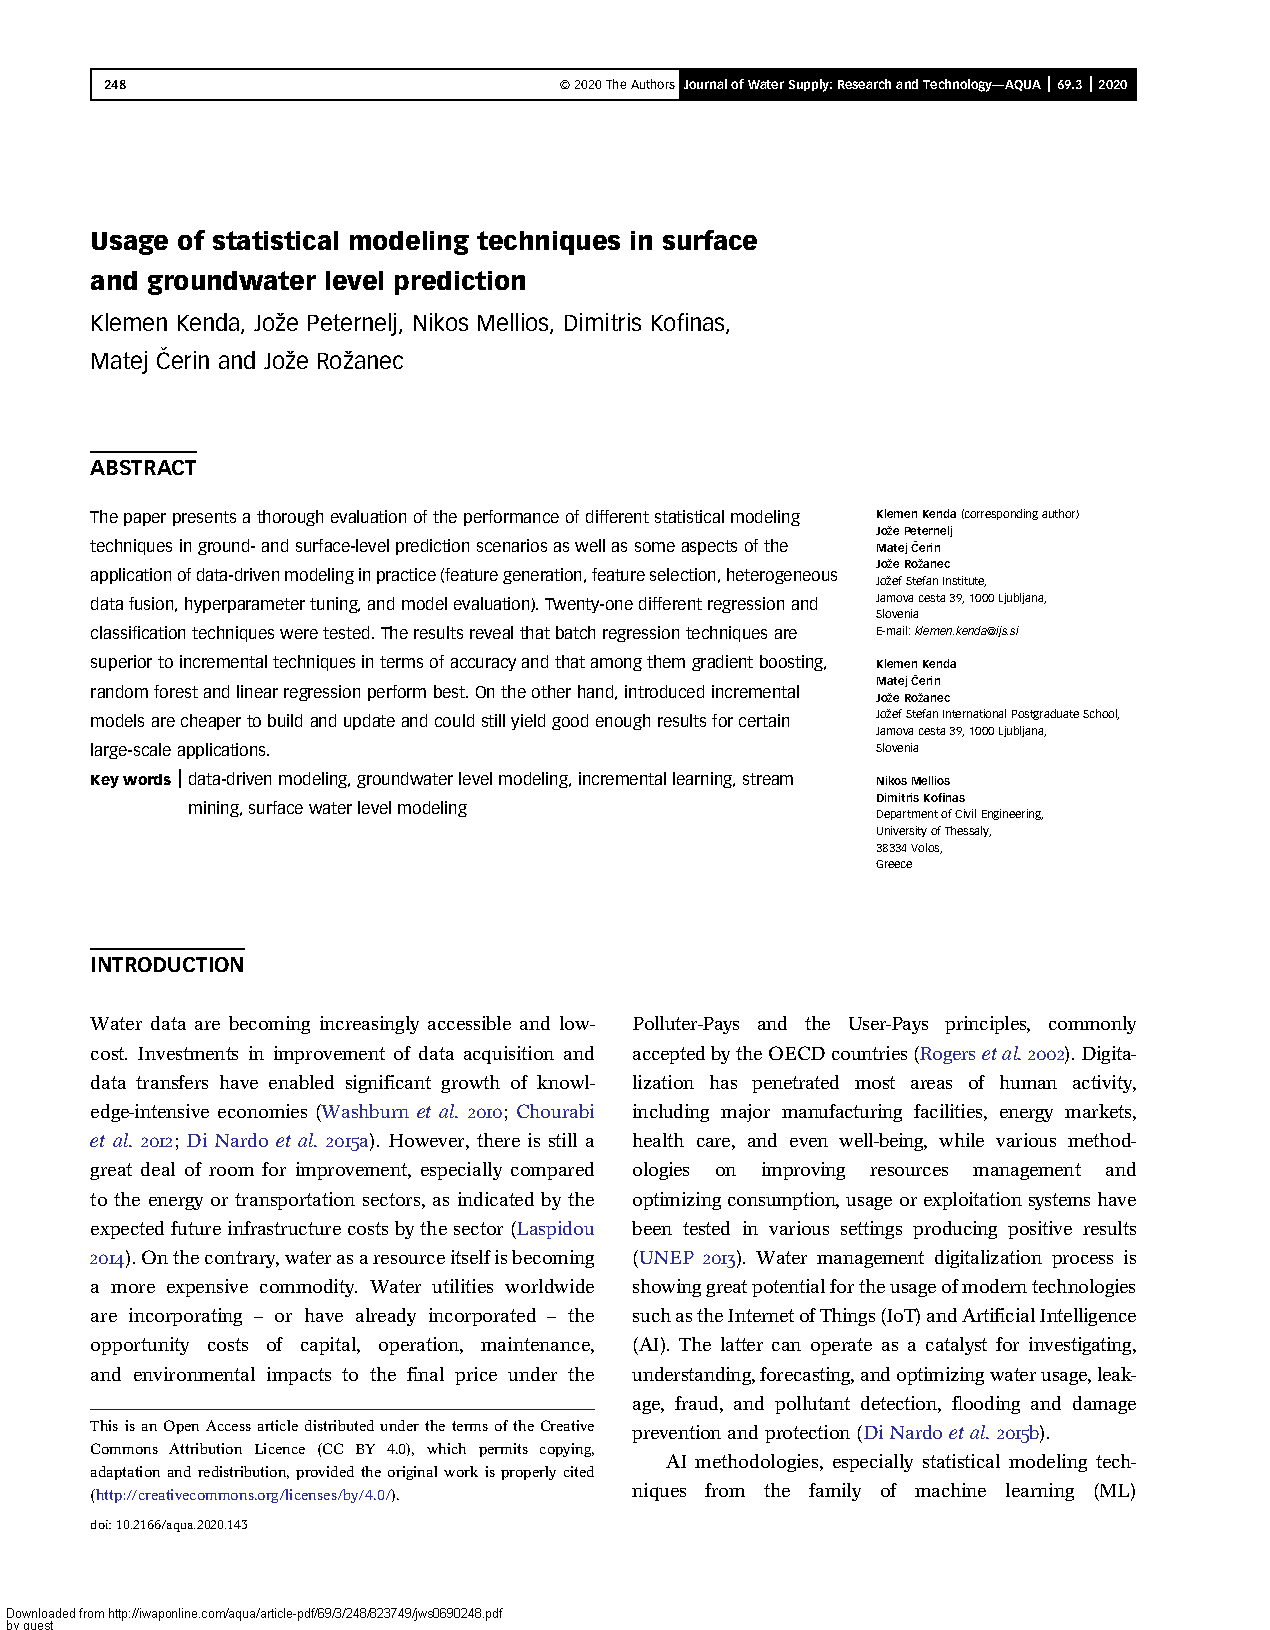
\includepdf[pages=-]{papers/water_level_prediction.pdf}